\asection{Methodology}
\label{Methodology}
\textbf{Primary Research Method:} Experiments
\textbf{Secondary Research Method:} Arguments

\setlistdepth{9}

\newlist{myEnumerate}{enumerate}{9}
\setlist[myEnumerate,1]{label=(\arabic*)}
\setlist[myEnumerate,2]{label=(\Roman*)}
\setlist[myEnumerate,3]{label=(\Alph*)}
\setlist[myEnumerate,4]{label=(\roman*)}
\setlist[myEnumerate,5]{label=(\alph*)}
\setlist[myEnumerate,6]{label=(\arabic*)}
\setlist[myEnumerate,7]{label=(\Roman*)}
\setlist[myEnumerate,8]{label=(\Alph*)}
\setlist[myEnumerate,9]{label=(\roman*)}

\subsection{Experiment}
\subsubsection{Data set}
The data set that is used in this experiment is a set of digraph objects of an arbitrarily large size. The digraphs that are used meet the following conditions
\begin{itemize}
  \item They are either partially or completely isomorphic in relation to one or other digraph inside the set.
  \item They are either partially,completely or not semantically similar to one or other digraph inside the set.
\end{itemize}

A quantitative approach is employed in evaluating the algorithms against each other. The search graph matching algorithms are implemented and experimented on, using two digraph objects at a time. The experiment for that is employed measure and records the algorithms ability and performance of the algorithms in cases where Graph A and Graph B are either partially or completely isomorphic, and cases where Graph A and B are partially, completely or not semantically similar.\\\\
A measure of the degree of similarity for both the syntactical and semantically similarity is calculated and recorded for each test case.

\subsubsection{Experiment implementation}

We will refer to Graph A and Graph B in this context.\\\\
The algorithm has to insert an arbitrarily large number of nodes.
\begin{myEnumerate}
  \item The two graph are compared to each other to evaluate the degree of their similarity.
  \item The comparison that is done is dependent on the relationship between Graph A and B.
		\begin{myEnumerate}
			\item \textbf{Syntactic comparison}					
				\begin{myEnumerate}
					\item Graph A is compared with the whole of Graph B for syntactical similarity.										
						\begin{myEnumerate}
							\item A new subgraph of Graph B is generated.
							\item The subgraph is compared with graph A for syntactical similarity.											
								\begin{myEnumerate}
									\item The time taken to perform the comparison is recorded.
									\item The amount of memory used by the algorithm to perform the comparison is recorded.
									\item The degree of syntactical(isomorphic) similarity is calculated relative to the graph of B and stored as well as the subgraph.						.
								\end{myEnumerate}	
							\item Once all the subgraphs of Graph B have been experimented upon, the result of the subgraph with the best degree of syntactical(isomorphic) similarity
									is recorded together with the subgraph.					
						\end{myEnumerate}
						
					\item If Graph A and B are not completely syntactically similar, Graph A is compared with all the possible subgraphs of Graph B.
				\end{myEnumerate}
				
			\item \textbf{Sementic comparison}
				\begin{myEnumerate}
					\item The sementic comparison is performed on Graphs that are Syntactically similar to some degree, this is because there is no point in comparing the sementics relationship of a Graphs if they are not even structurally the same.
						\begin{myEnumerate}
							\item If the syntactical similarity of Graph A and Graph B is equal to 1.0, then...
								\begin{myEnumerate}
									\item Graph A is compared with the whole of Graph B for semantical similarity.
										\begin{myEnumerate}
											 \item The time taken to perform the comparison is recorded.
											 \item The amount of memory used by the algorithm to perform the comparison is recorded.
											 \item The degree of semantical(isomorphic) similarity is recorded.											
										\end{myEnumerate}
								\end{myEnumerate}
							\item If the syntactical similarity of Graph A and Graph B is a fraction of 1.0, then...
								\begin{myEnumerate}
									\item Graph A is compared with all the possible subgraphs of Graph B.
										\begin{myEnumerate}										
										  \item The subgraph that was recorded during the Syntactic comparison is retrieved.
										  \item The subgraph is compared with graph A for semantical similarity.
											\begin{myEnumerate}
												\item The time taken to perform the comparison is recorded.
												\item The amount of memory used by the algorithm to perform the comparison is recorded.
												 \item The degree of semantical(isomorphic) similarity is calculated relative to the graph of B and recorded as well as the subgraph.
											\end{myEnumerate}
										\end{myEnumerate}
								\end{myEnumerate}
						\end{myEnumerate}
				\end{myEnumerate}
		\end{myEnumerate}
\end{myEnumerate}

\break

\textbf{\underline{Calculating the Syntactic and Sementical similarities}}\\\\
The Syntactic and Sementical similarities are a calculated relative to some graph, and they both use the same function.\\
The funation calculates all the nodes in the reference graph, and they are divided by the number of nodes inside the subgraph.\\
Example.
\begin{figure}[H]
\centering
\begin{subfigure}{.5\textwidth}
  \centering
  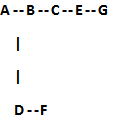
\includegraphics[width=.4\linewidth]{GraphA.PNG}
  \caption{Reference Graph}
\end{subfigure}%
\begin{subfigure}{.5\textwidth}
  \centering
  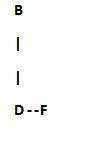
\includegraphics[width=.4\linewidth]{GraphB.PNG}
  \caption{Sub graph}
\end{subfigure}
\caption{A figure with two graphs that are used to demonstrate the calculation}
\label{fig:test}
\end{figure}

\textbf{\textit{Similarity = 3/7 = 0.429 units.}}\\

\subsection{Experiment}
The recorded results from all the algorithms is analyzed and used to identify which amongst the algorithms is the best and for which cases it is the best in.\\
The results from the algorithms are weighed against a comparison criteria, and it is this criteria that is used to evaluate the algorithms against each other.\\

\subsubsection{The comparison criteria}
The criteria that the algorithm results are weighed against is specified below.
\begin{myEnumerate}
	\item Space efficiency
	\item Complexity of the algorithm
	\item Degree of synactical similarity result generated by the algorithm per test case.
	\item Degree of sementical similarity result generated by the algorithm per test case.
 \end{myEnumerate}
 \break
 
Once the results have been obtained and throughly evaluated, then the algorithms with the best perform per criteria field are recorded.\\
And from that set, the best algorithm is chosen overall relative to the others based on the criteria.